%\newpage
%\section{Заполнение шаблона}
%\begin{itemize}
	%\item Изменить \textbf{config.tex}: имя студента, название предмета и пр. %параметры указаны именно там
	%\item Заполнить \textbf{content.tex} - файл, который будет содержать весь %текст отчёта, от вступления до заключения.
	%\item Добавить используемую литературу (если есть) в \textbf{refs.bib}. Для %удобного поиска источников можно воспользоваться Google Books. Использованные %источники можно указывать с помощью команды \textbf{\\cite\{name\_of\_ref\}}
%\end{itemize}
%Далее представлены различные примеры.

\section{Цель работы}\label{sec:purpose}


Определить состав образцов по полученным спектрам люминесценции и возбуждения люминесценции.

\section{Задачи, решаемые в лабораторной работе}\label{sec:tasks}
\begin{enumerate}
	\item Снять спектры люминесценции и возбуждения люминесценции исследуемых образцов.
	\item Определить по полученным спектрам, какие ионы (атомы) являются центрами свечения в данных образцах.
\end{enumerate}

\section{Объект исследования}\label{sec:object}

Оптические материалы неизвестного состава.
%\section{Теоретическая информация}\label{sec:теоретическая-информация}

%Было использовано методическое указание по выполнению лабораторного практикума по основам фотоники.
%Исследование кинетических свойств фотохромных стекол~\cite{conlan1983massive}.

%\section{Рабочие формулы и исходные данные}\label{sec:initial_data}

%\begin{equation}
%a= \begin{cases}
% 3x + 5y + z, \mbox{если хорошо} \\
% 7x - 2y + 4z, \mbox{если плохо}\\
% -6x + 3y + 2z, \mbox{если совсем плохо}
%\end{cases}
%\label{eq:F10}
%\end{equation}

%\begin{equation}
%\tau{_{rad}^{-1}} = 8 \cdot \pi \cdot c
%					\cdot n^2 \cdot \tilde{\nu}^2 \cdot \frac{8}{7}
%					\cdot \int \sigma_{abs}(\nu)d\nu
%\label{eq:F1}
%\end{equation}
%где $c$ – скорость света, $n$ – показатель преломления стекла,
%$\tilde{\nu}$ – средняя частота полосы, $\int \sigma_{abs}(\nu)d\nu$
%– интегральное сечение поглощение основного
%резонансного перехода
%${}^4$$I_{15/2}\rightarrow{}^4$$I_{13/2}$
%
%%\rightarrow\sideset{^4}{_{13/2}}I
%\begin{equation}
%q = (\tau_{exp}/\tau_{rad}) \cdot 100\%,
%\label{eq:F2}
%\end{equation}
%где $\tau_{exp}$ – экспериментально определенное время
%жизни люминесценции перехода
%${}^4$$I_{15/2}\rightarrow{}^4$$I_{13/2}$,
%$\tau_{rad}$ – радиационное время жизни люминесценции перехода
%${}^4$$I_{15/2}\rightarrow{}^4$$I_{13/2}$.

%\section{Оборудования и принадлежности}\label{sec:stuff}
%\subsection{Схема установки}\label{subsec:schemes}
%\begin{figure}[H]
%        \centering
%        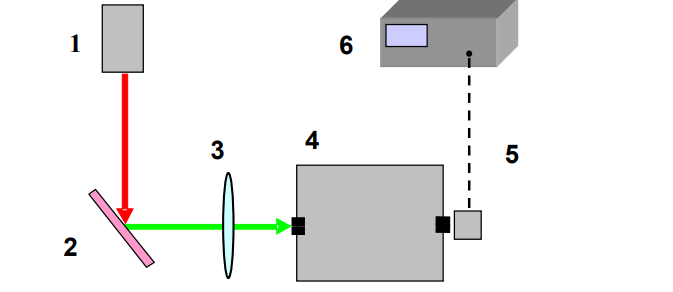
\includegraphics[width=0.7\columnwidth]{figures/Scheme}%[width=]
%        \caption{Схема установки для определения кинетики затухания
%люминесценции. Цифрами на схеме обозначены: (1) – импульсный лазер; (2)
%– образец; (3) – короткофокусный объектив; (4) – монохроматор; (5) –
%InGaAs-приемник (6) –осциллограф}
%		\label{fig:Scheme}
%\end{figure}
\section{Результаты эксперимента}\label{sec:results}

Построили спектр интенсивности и
люминесценции от времени для каждого образца.
\begin{figure}[H]
	\centering
	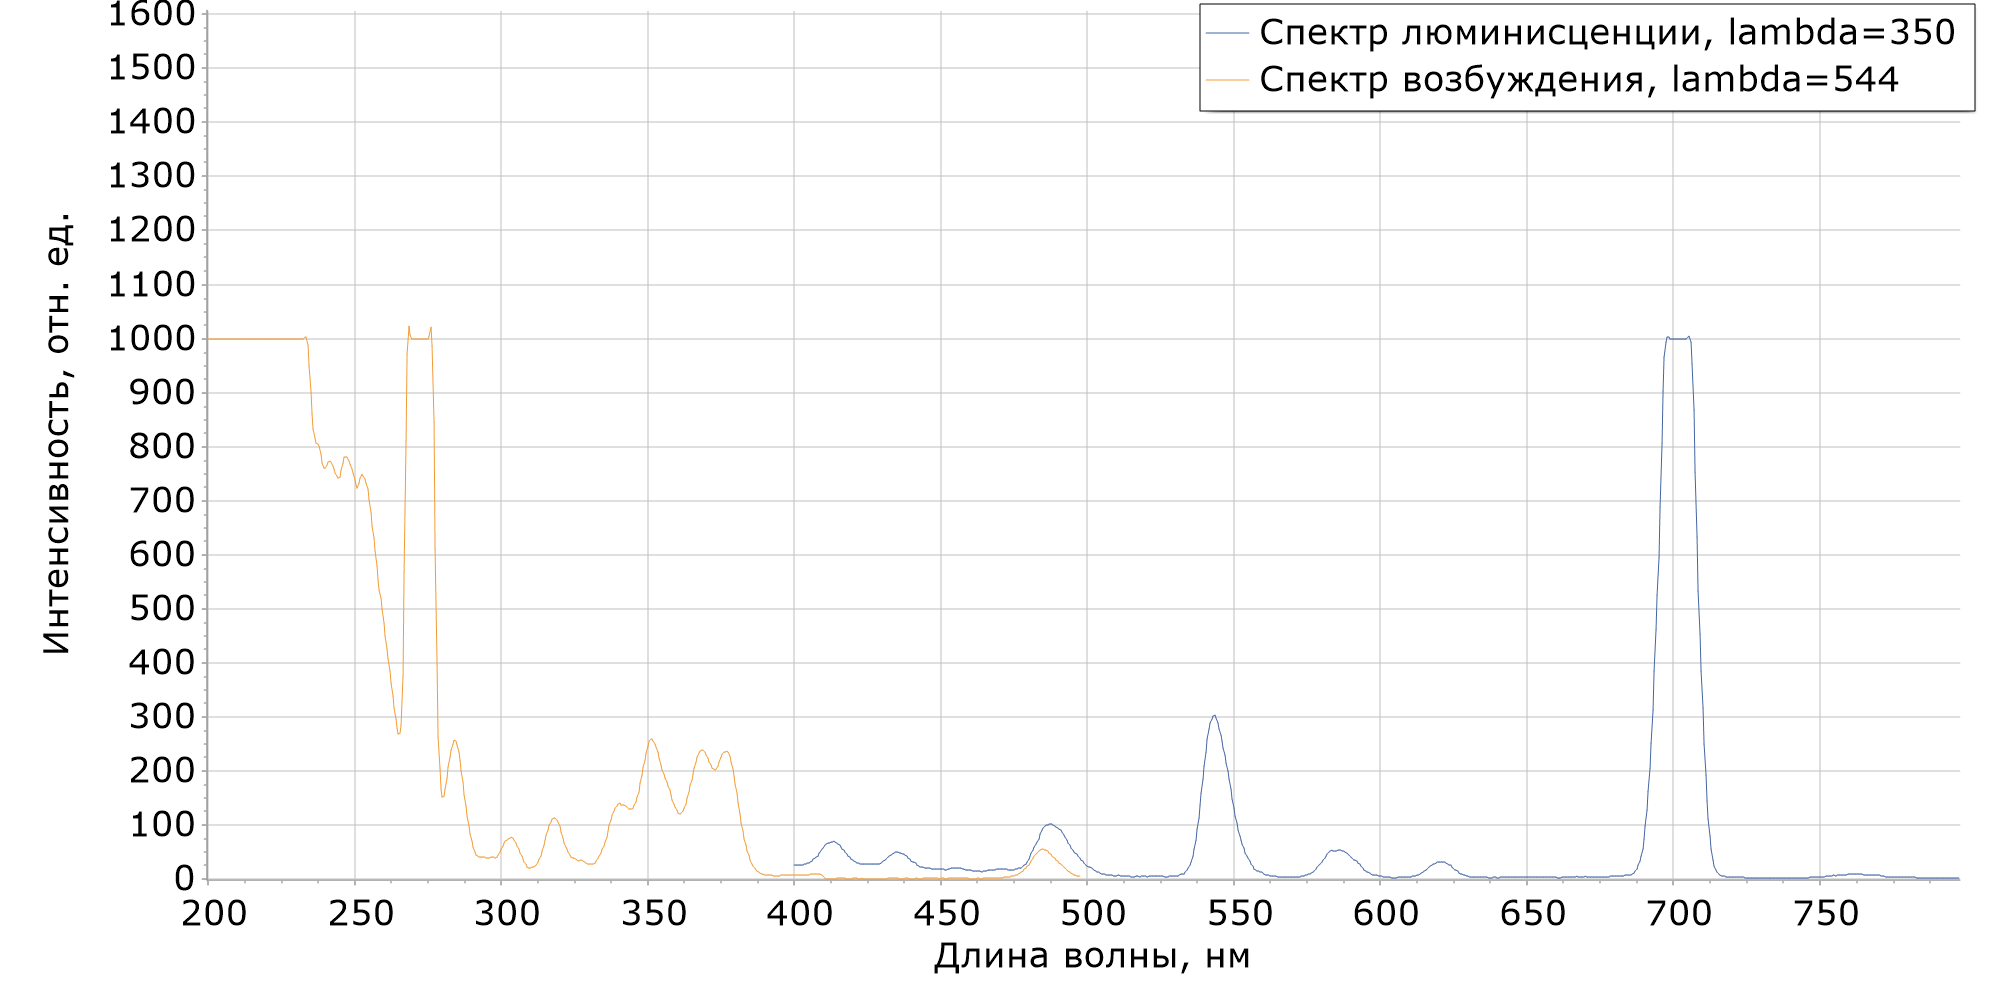
\includegraphics[width=7in]{figures/Obr_1}
	\caption{Спектры люминесценции и возбуждения люминесценции образца №1}
	\label{fig:Lum1}
\end{figure}

\begin{figure}[H]
	\centering
	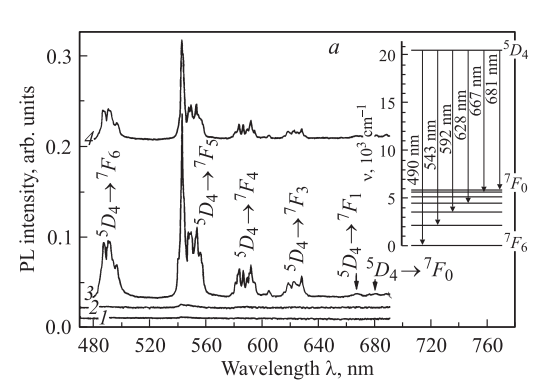
\includegraphics[width=5in]{figures/img}
	\caption{Спектры люминесценции Tb3+\cite{AfotoTB3}}
	\label{fig:LumTb}
\end{figure}

Центром свечения для образца 1 вероятнее всего выступает тербий.
Это следует из совпадения основных пиков для люминисценции тербия.
На графике \ref{fig:LumTb}, указаны переходы, соответствующие иону Tb3+.

\begin{figure}[H]
	\centering
	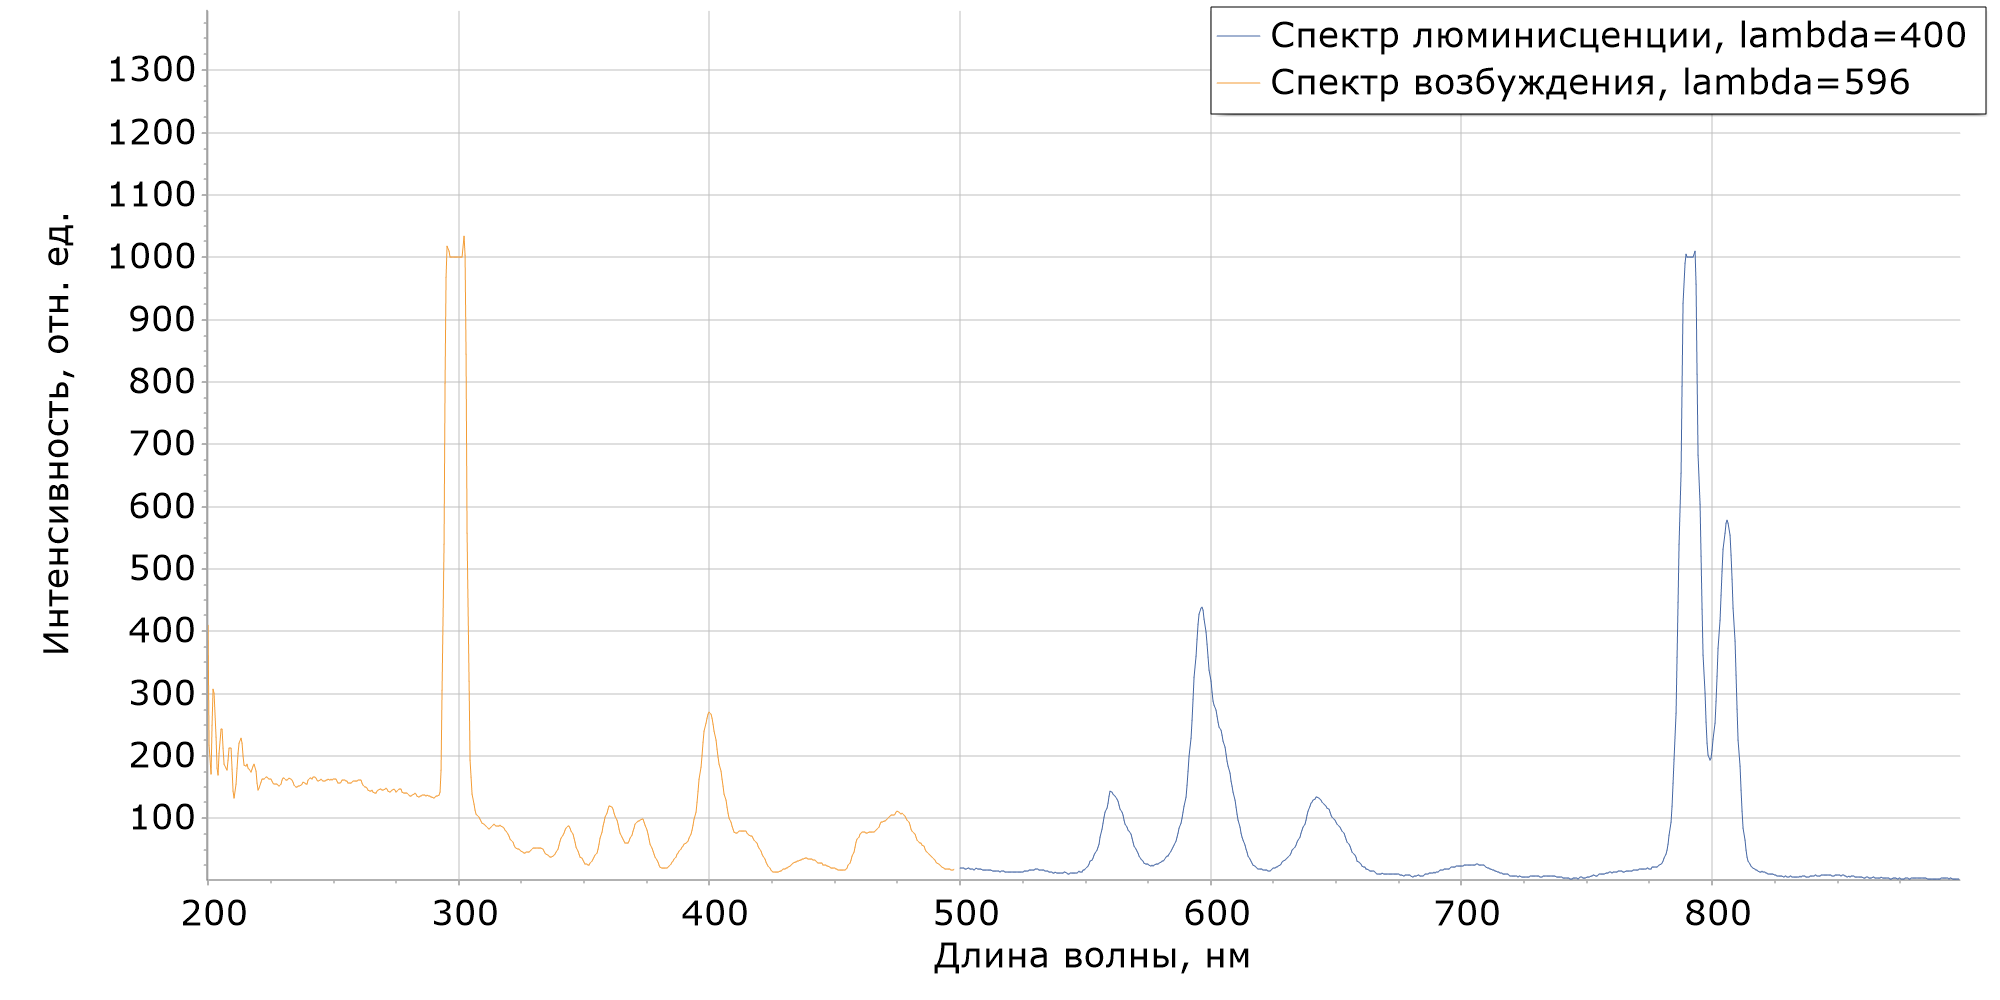
\includegraphics[width=7in]{figures/Obr_2}
	\caption{Спектры люминесценции и возбуждения люминесценции образца №2}
	\label{fig:Lum2}
\end{figure}

\begin{figure}[H]
	\centering
	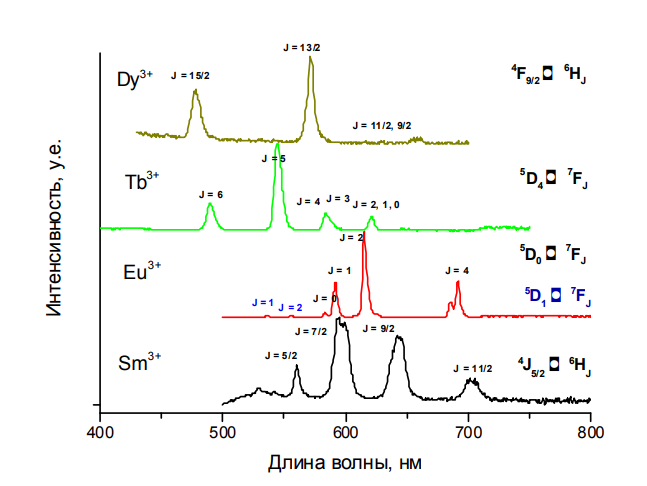
\includegraphics[width=5in]{figures/img_1}
	\caption{Спектры люминесценции Sm3+\cite{BSpecCourse}}
	\label{fig:LumSum}
\end{figure}

Анализируя график \ref{fig:Lum2}, можно сделать вывод, что
центром свечения для образца 2 вероятнее всего выступает самарий.
На графике \ref{fig:LumSum} указаны переходы, соответствующие иону Sm3+.

\begin{figure}[H]
	\centering
	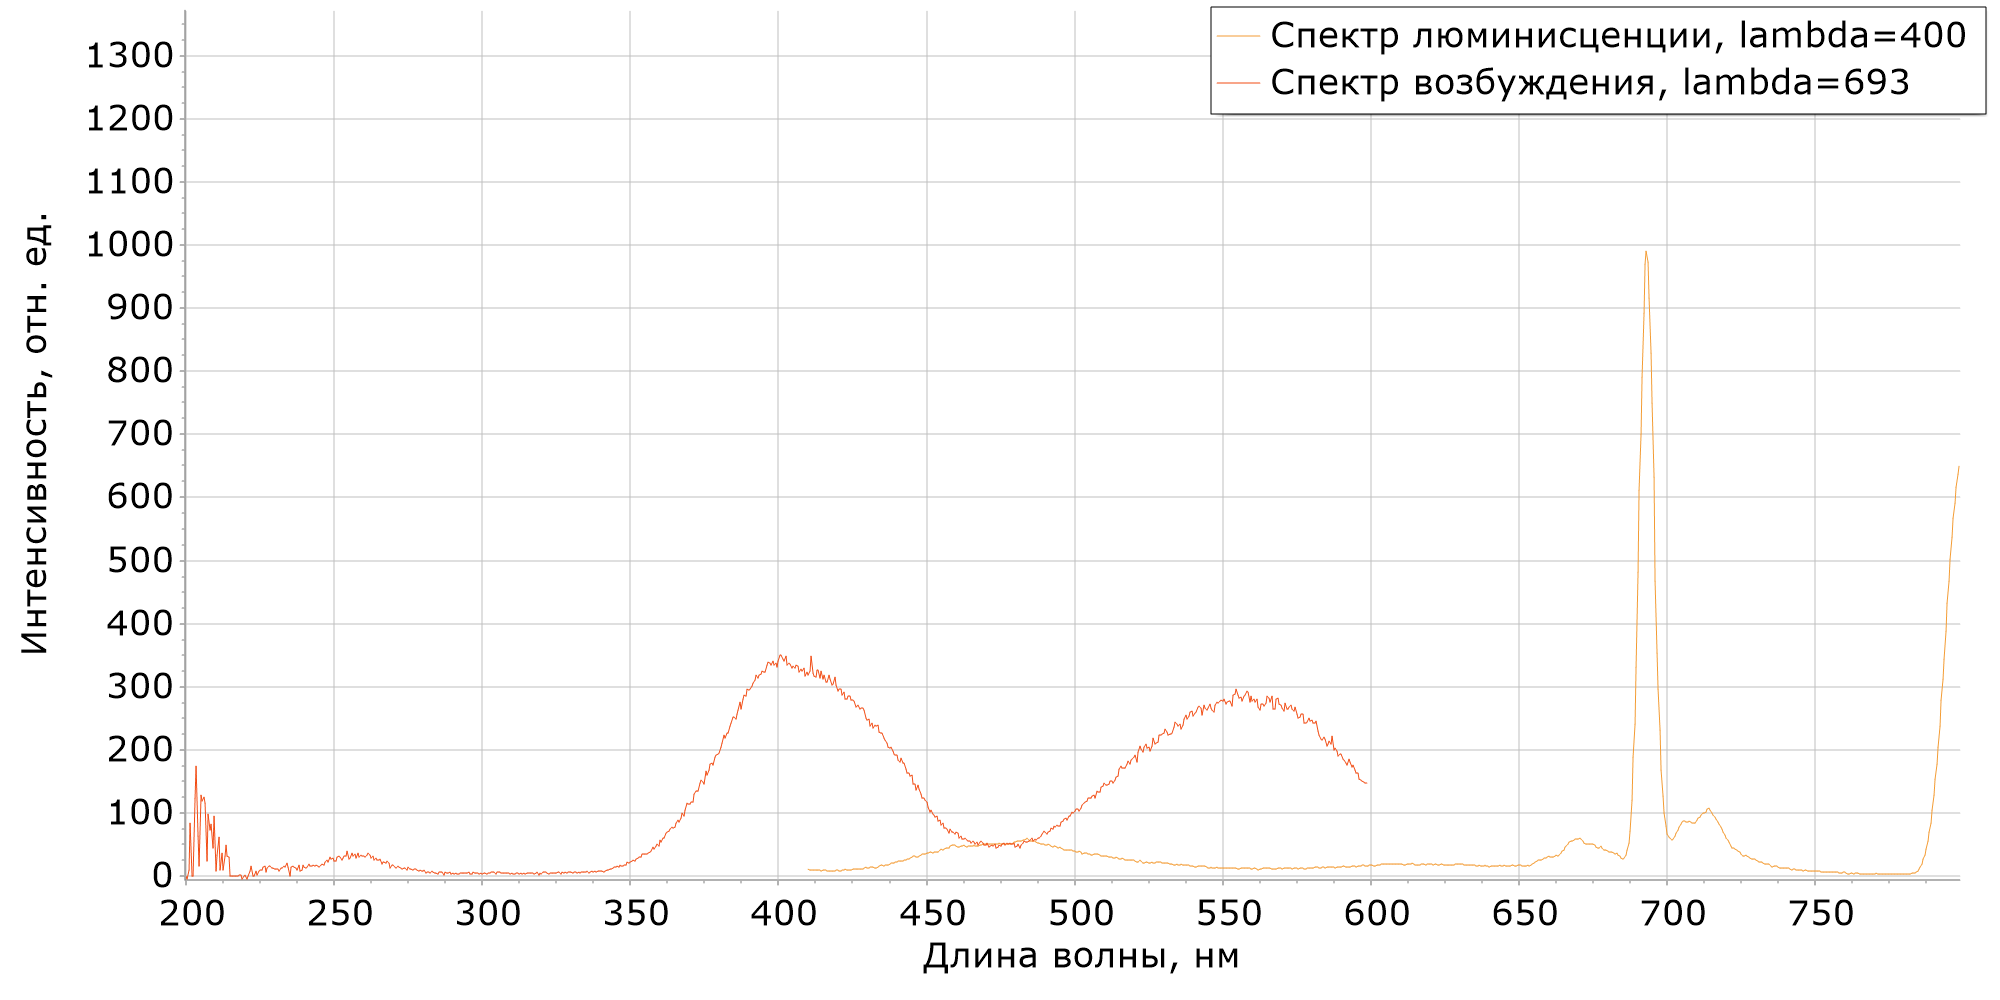
\includegraphics[width=7in]{figures/Obr_3}
	\caption{Спектры люминесценции и возбуждения люминесценции образца №3}
	\label{fig:Lum3}
\end{figure}

\begin{figure}[H]
	\centering
	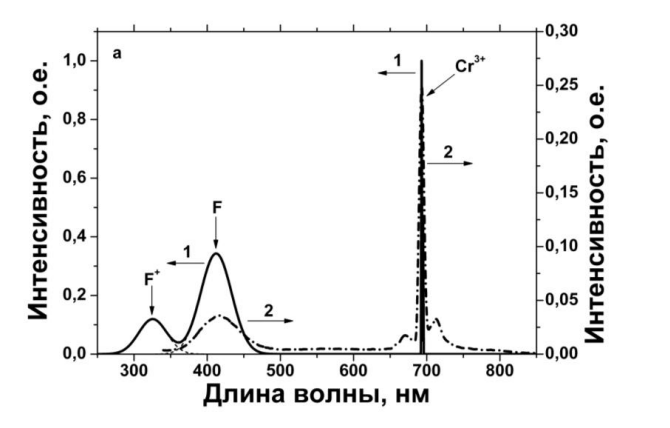
\includegraphics[width=5in]{figures/img_2}
	\caption{Спектры люминесценции Cr3+\cite{CShtang}}
	\label{fig:LumCr}
\end{figure}

Анализируя график \ref{fig:Lum3}, можно сделать вывод, что
центром свечения для образца 3 вероятнее всего выступает хром.
На графике \ref{fig:LumCr} указан спектр люминисценции, соответствующий керамике оксида алюминия с ультрадисперсной структурой с центром люминисценции Cr3+.

\begin{figure}[H]
	\centering
	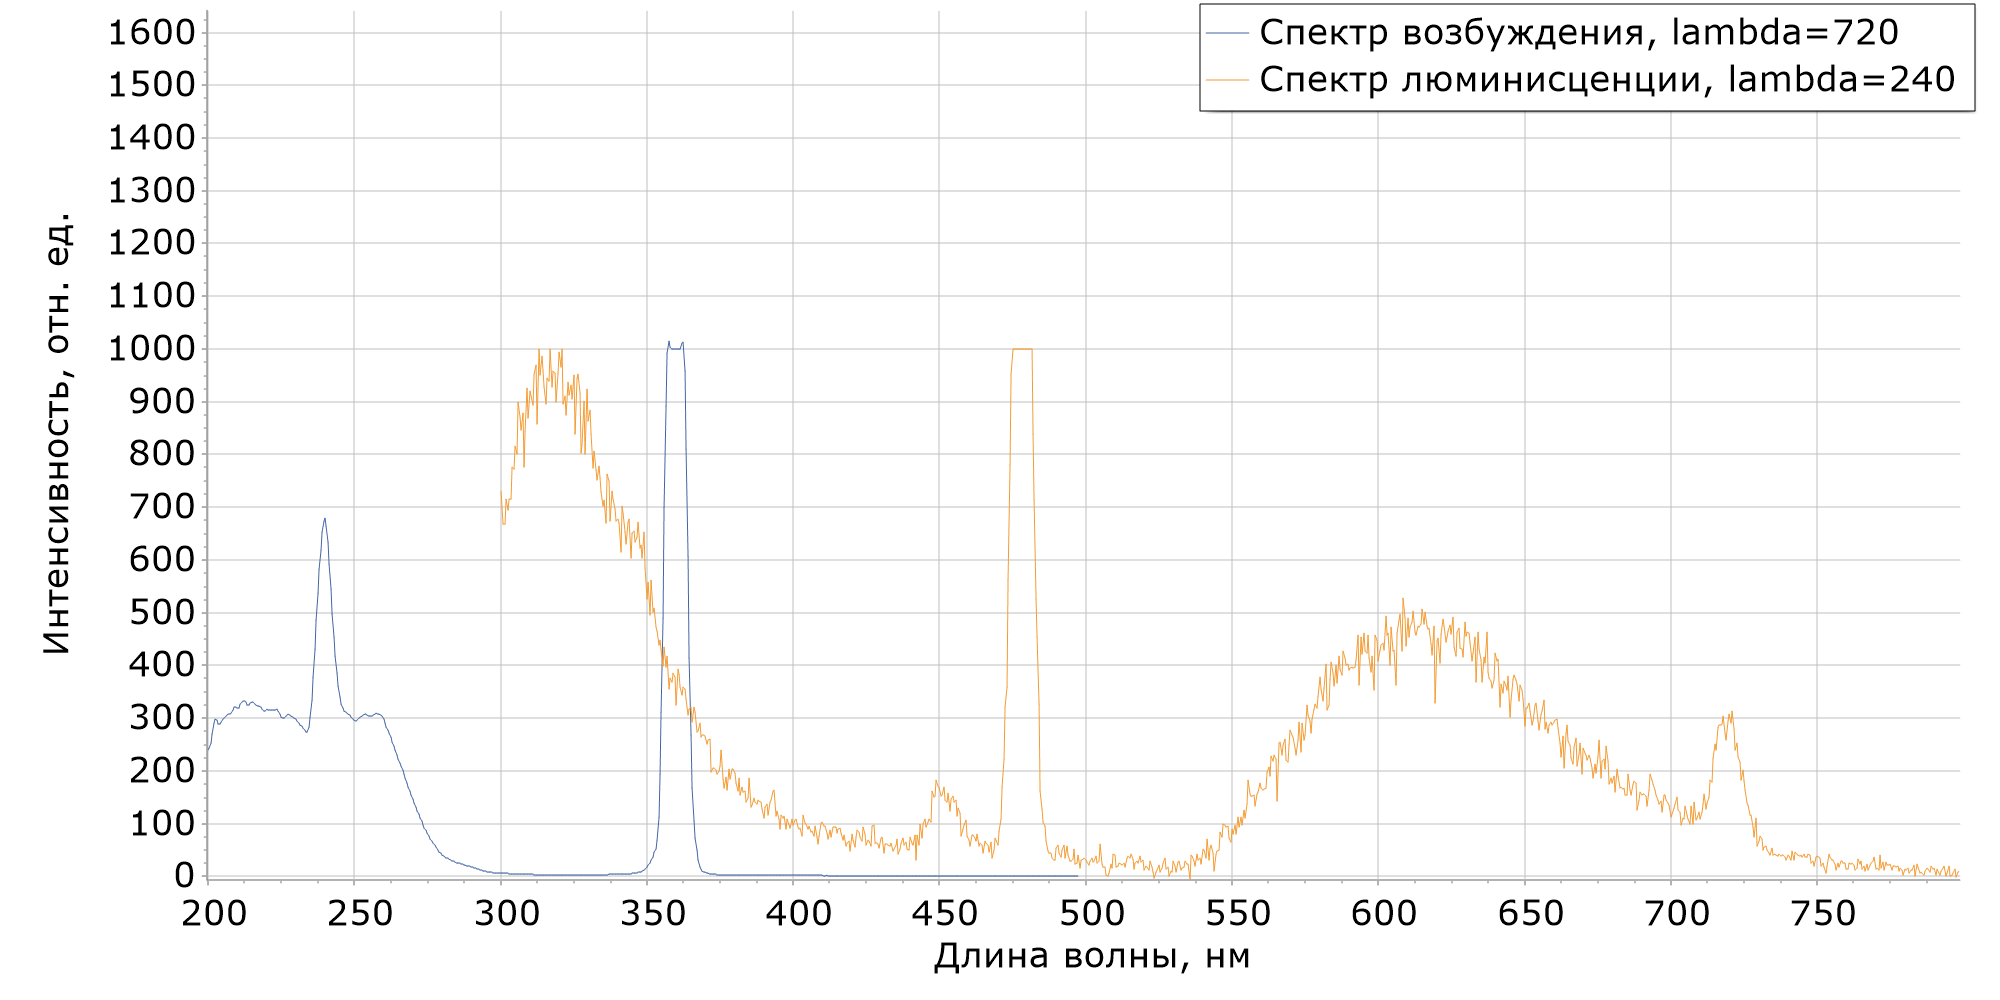
\includegraphics[width=7in]{figures/Obr_4}
	\caption{Спектры люминесценции и возбуждения люминесценции образца №4}
	\label{fig:Lum4}
\end{figure}

Анализируя график \ref{fig:Lum4}, можно предположить, что
центром свечения для образца 4 вероятнее всего выступает смесь Европия(Eu) и чего-то еще.

% Please add the following required packages to your document preamble:
% \usepackage{multirow}
% \usepackage{graphicx}
%\begin{table}
%    \centering
%	\begin{threeparttable}% выравнивание подписи по границам таблицы
%    % \captionsetup{justification=raggedright} % выравнивание подписи по-центру
%    \caption{Основные величины СИ}\label{tab:unit:base}
%    \begin{tabular}{llc}
%        Название  & Команда                 & Символ         \\
%        Ампер     & 12 & затухания   люминесценции, мсзатухания   люминесценции,   \\
%        Кандела   & 123 & 1123 \\
%        Кельвин   & 123 & 123   \\
%        Килограмм & 123 & 123 \\
%        Метр      & 123 & 123    \\
%        Моль      & 123 & 123     \\
%        Секунда   & 123 & 123   \\
%    \end{tabular}
%	\end{threeparttable}
%\end{table}

\section{Выводы и анализы результатов}\label{sec:conclution}

В ходе выполнения данной лабораторной работы были сняты спектры люминесценции и возбуждения образцов, по виду которых были определены ионы, обеспечивающие люминесцентные свойства.

Установленные параметры для спектрофлуориметра оказались оптимальными.
Ширина щели 5 мкм позволяла получать достаточные интенсивности для определения пиков люминесценции.
Однако неподходящая скорость измерения для образца №2 и №4 привела к появлению шумов, мешающих определению линий в спектре.

Длины волн излучения для снятия спектра люминесценции выбирались по наиболее активному отклику образца на подаваемое излучения.
Для спектра возбуждения люминесценции - по максимальному пику в спектре люминесценции для исследуемого образца.
В процессе измерений не были использованы фильтры, что привело к появлению второго порядка дифракции, приводящий к зашкаливающим линиям на спектре.

Для всех образцов, кроме 4-го удалось определить какие ионы (атомы) являются центрами свечения.

